\chapter{Motivation}\label{blabli}
Code: \url{https://github.com/NeverL8/ADL/tree/main/B08}
\vspace{0.75cm}\newline

A striking feature of transformer networks is the aspect of self-attention: The input has variable length and all elements have attention to the other input elements.
A representation learnt from information combination is then used to perform a prediction.
So: The weights for each input are not fixed after training which was the case for our previous models.Here, we will apply a transformer network to the IceCube 2D dataset.
The IceCube dataset contains separate training, validation and testing files. From 3D input (time and two spatial orientations) of a series of hits belonging
to an event (neutrino interaction) the interaction position is predicted. In this case self-attention can e.g. help reduce the effect of noise, as attention (weight) is given to correlated hits.

The same exercise has been done using a Graph Neural Network (GNN). A brief comparison of the results of both models will follow in this report.
\chapter{Code architecture}
For most parts of the code, previously used code (e.g. for training, evaluation, (de-)normalisation) as well as the template given (transformer structure and padding) have been adjusted and reused.
Before applying a transformer layer the 3D input is transformed into a richer higher-dimensional representation in a first linear layer.
The following transformer layer consists of a multi-head attention block followed by a small MLP.
Both components are connected by skip connections and layer normalization.
Multiple attention heads are used in order to focus on several attention patterns.
The transformer itself is not coded here, but simply called using TransformerEncoder and TransformerEncoderLayer respectively.
Only the network parameters have to be given when calling the class. These are the network parameters that I used:
\begin{minted}{python}
hidden_dim=128,
nhead=4,          
num_layers=3,    
dim_feedforward=128
\end{minted}
On a technical note: We should ideally have identical length input for all events for efficient per-batch calculation. In order to account for variable-length input, padding has to be used: We find the length of the longest input series and increase
all other input lengths to the same length. The additional hits are marked as faked via an additional mask which 
ensures that only valid hits influence the prediction derived after applying mean-pooling.

For training we use the following hyperparameters:
\begin{minted}{python}
batch_size = 32
criterion = nn.MSELoss()
optimizer = optim.Adam(model.parameters(), lr=0.002, weight_decay=1e-5)
\end{minted}
Normalisation is done via standardisation, just like for the GNN exercise.

\chapter{Results and observations}
As displayed in \autoref{loss}, training quickly converges, but there still seems to be room for loss reduction after longer training. In different runs with slightly different hyperparameters loss has saturated earlier already (not shown here).
\begin{figure}[h]
    \centering
    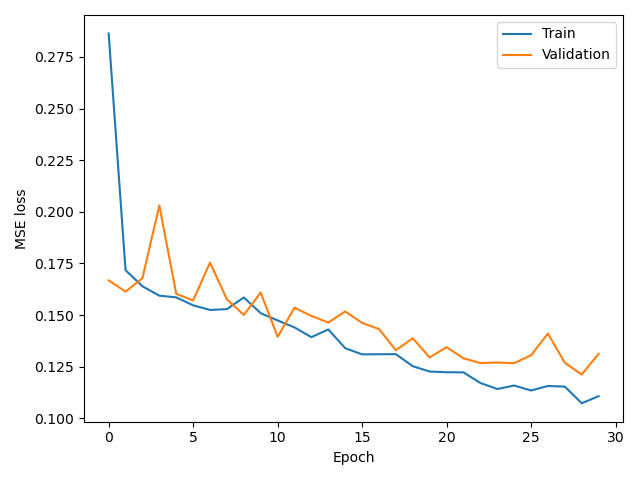
\includegraphics[width=0.7\textwidth]{../images/loss.png}
    \caption{Loss curves.}\label{loss}
\end{figure}
In \autoref{comparison_trans} we compare true and predicted $x$ and $y$ coordinates for the transformer predictions.
The overall variance seems to be quite large and there is a slight bias. One can see that
$x$ predictions tend to be slighly overestimated as $y$ predictions tend to be underestimated.
\begin{figure}[htbp]%
    \centering%
%
    \begin{subfigure}{0.5\textwidth}%
        \centering%
        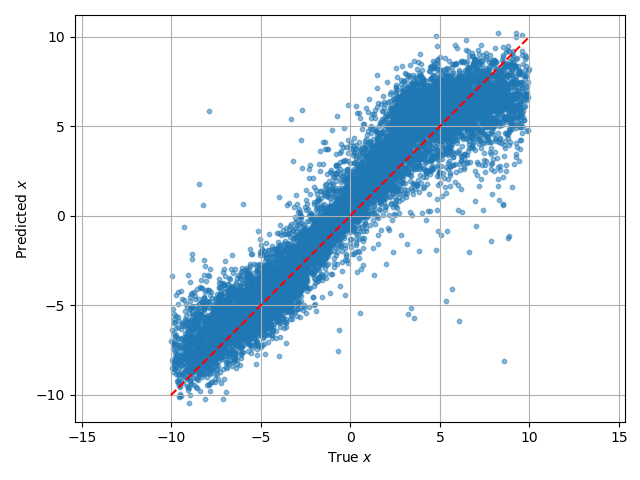
\includegraphics[width=\linewidth]{../images/true_vs_predicted_x.png}%
        \caption{$x$.}%
    \end{subfigure}%
%
    %\vspace{1em}
%
    \begin{subfigure}{0.5\textwidth}%
        \centering%
        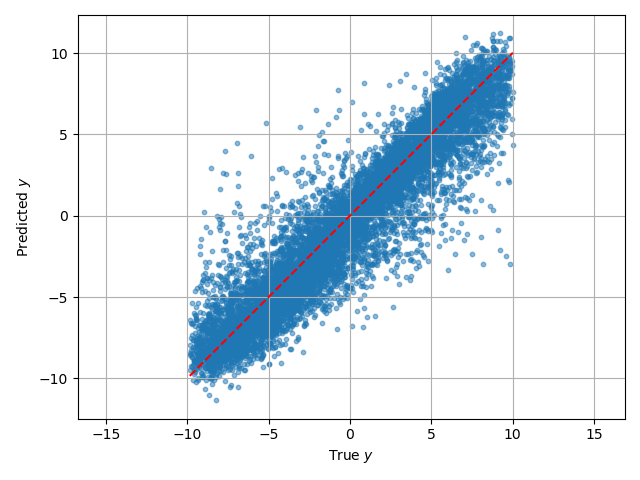
\includegraphics[width=\linewidth]{../images/true_vs_predicted_y.png}%
        \caption{$y$.}%
    \end{subfigure}%
\caption{True vs predicted coordinates for the transformer model.}\label{comparison_trans}%
%
\end{figure}
Contrarily, we have seen a clear bias for GNNs, especially for large $x$ (see \autoref{comparison_GNN}).
\begin{figure}[htbp]
    \centering%
%
    \begin{subfigure}{0.5\textwidth}%
        \centering%
        \includegraphics[width=\linewidth]{../../B04/output.png}%
        \caption{$x$.}%
    \end{subfigure}%
%
    %\vspace{1em}
%
    \begin{subfigure}{0.5\textwidth}%
        \centering%
        \includegraphics[width=\linewidth]{../../B04/output_y.png}%
        \caption{$y$.}%
    \end{subfigure}%
\caption{True vs predicted coordinates for the GNN model.}\label{comparison_GNN}%
%
\end{figure}
When looking at the overall prediction heat maps, both GNN and transformer exhibit a similar pattern: While the
true distribution is somewhat uniform within a circle, both prediction maps show an accumulation for large $x$ and $y\approx0$.
Darker spots can be observed at $x\approx\pm2.5$.
\begin{figure}[htbp]
    \centering%
%
    \begin{subfigure}{0.5\textwidth}%
        \centering%
        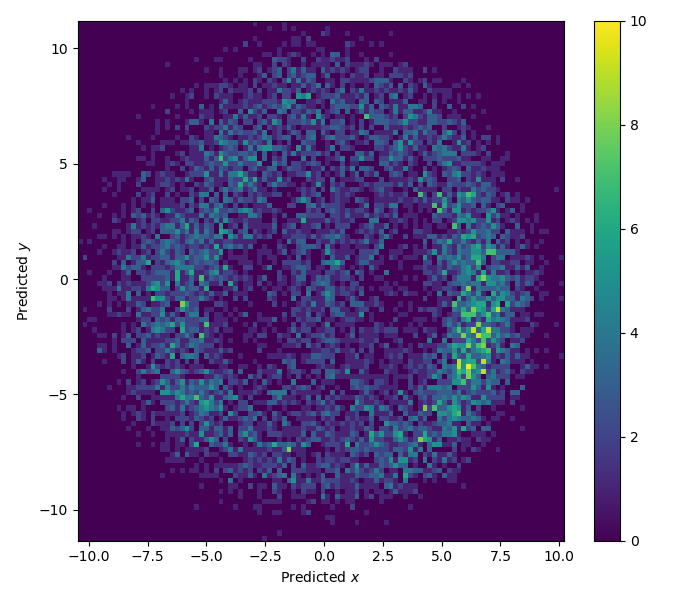
\includegraphics[width=\linewidth]{../images/predictionMap.png}%
        \caption{Transformer network.}%
    \end{subfigure}%
%
    %\vspace{1em}
%
    \begin{subfigure}{0.5\textwidth}%
        \centering%
        \includegraphics[width=\linewidth]{../../B04/heatmap.png}%
        \caption{GNN.}%
    \end{subfigure}%
\caption{Predicted interaction locations.}\label{comparison_heat}%
%
\end{figure}
The error distribution is shown in \autoref{distance}.
\begin{figure}[h]
    \centering
    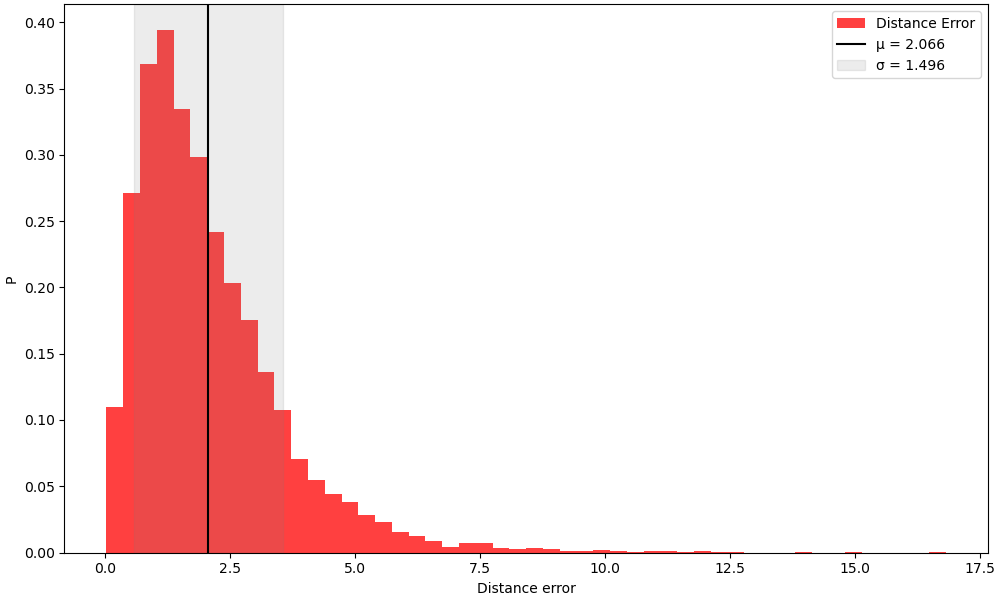
\includegraphics[width=0.7\textwidth]{../images/deviations.png}
    \caption{Histogram of Euclidian distance between truth and prediction for the transformer network.}\label{distance}
\end{figure}
Comparing the mean and median Euclidian distance between truth and prediction also shows similar results for the GNN and transformer network:
\begin{align*}
    &\textbf{Transformer:}\\
    &\text{Mean reconstruction error: } 2.0663235\\
&\text{Median reconstruction error: } 1.7184832\\
    &\textbf{GNN:}\\
    &\text{Mean reconstruction error: } 2.0202744\\
&\text{Median reconstruction error: } 1.7047672\\
\end{align*}
\chapter{Conclusion}
Since the same patterns in prediction maps occur for both network architectures, these occurences are likely (fortunately) not introduced by the network, but rather linked to the data itself:
The histograms of all three datasets look similar for both $x$ and $y$ coordinates (not shown here).
All distributions are roughly symmetric with the occurence of interactions becoming rarer towards the edges.
Hence, there definitely are weaker statistics for detector hits close to the edges. However, the aforementioned biases likely
stem from the individual hits for each interaction. The direction of travel as well as the variance in $x$ and $y$ direction likely
influence prediction accuracy.
Slight, non-systematic variation of transformer hyperparameters has been tested (not shown here), but the bias consists for each set of hyperparameters.

Since GNNs also take neighbours in feature space into account, one can presume that they provide excellent predictions for this application.
Unfortunately, despite the complexity of the network, the transformer model seems to perform similarly well as the GNN model for this exercise.